\documentclass[10pt,a4paper]{article}
\usepackage[latin1]{inputenc}
\usepackage{amsmath}
\usepackage{amsfonts}
\usepackage{amssymb}
\usepackage{graphicx}
\usepackage{fullpage}
\usepackage{float}

\title{DD2424 Lab 1}
\author{Artem Los (arteml@kth.se)}
\date{\today}

\begin{document}

\maketitle

\section*{Introduction}
In this lab, we will implement a simple 1-layer network and train it on the CIFAR-10 dataset (sample from the data set shown below).

\begin{figure}[H]
	\centering
	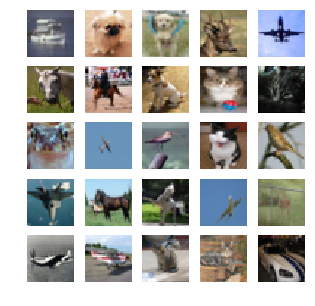
\includegraphics[width=5cm]{img/randompics.png}
\end{figure}

\section*{Tests for analytical gradient}
In order to test the correctness of analytical gradients, numerical gradients were used. We developed a function called \verb|checks|, which computes both the numerical and analytical gradients. For analytical gradients, batch size and the number of epochs are set to $1$ with no regression (i.e. $\lambda=0$).

To compare these gradients, we used the function \verb|grad_diff| (which computes the relative error between the numerical and analytical gradients). We concluded that the relative error was small (in the order of $10^{-8}$ for $W$ and $10^{-1}$ for $b$) and this did not change significantly as we increased the sample size.

Moreover, with the right configuration of hyperparameters, similar error values were observed as those presented in the lab instructions.

\section*{Results}
A summary of the results is found in Table \ref{results},\ref{lossvsepochs},\ref{weights}. From the results, especially Table \ref{lossvsepochs}, one can see that increasing the amount of regularization makes the training and test loss more similar and smoother, when comparing the the top (without regularization) vs. bottom (with regularization) images. From the same table, we can observe that having a very large learning rate will increase the number of spikes in the graph and in some cases may not lead to convergence (as seen in top-left image).

\begin{figure}[H]
\centering
\begin{tabular}{|llll|}
\hline
Lambda & Eta & Training error & Test error \\
\hline
0 &  0.1 & 0.1844 & 0.1705\\ 
0 & 0.01 & 0.4149 & 0.3685\\
0.1 & 0.01 & 0.3417 & 0.3338\\
1 & 0.01 & 0.2223 & 0.2173 \\
\hline
\end{tabular}
\caption{Training and test error for each set of hyperparameters used during training (with $epochs=40,n\_batch=100$).}
\label{results}
\end{figure}

\begin{figure}[H]
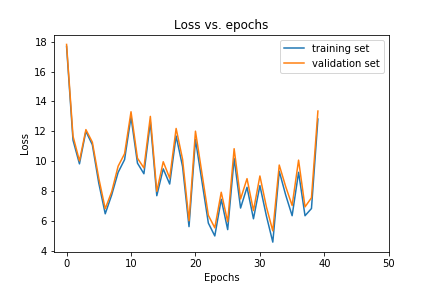
\includegraphics[width=7.5cm]{img/training1.png}
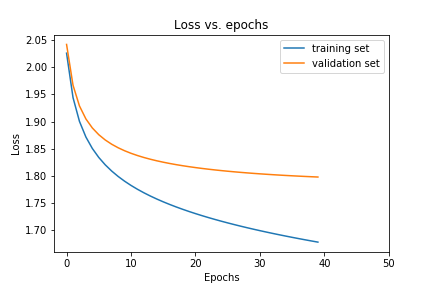
\includegraphics[width=7.5cm]{img/training2.png}\\
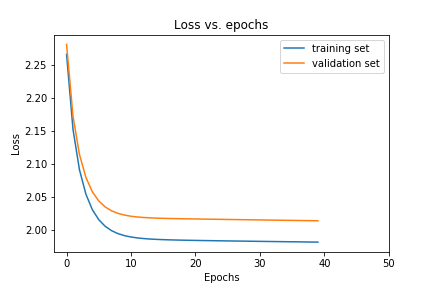
\includegraphics[width=7.5cm]{img/training3.png}
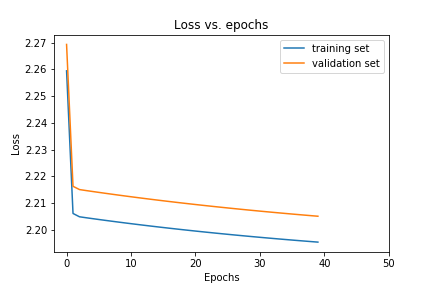
\includegraphics[width=7.5cm]{img/training4.png}
\caption{The loss vs. the number of epochs for each set of hyperparameters in \ref{results}. Row 1-2 are the top images (from left to right in ascending order), and row 3-4 are at the bottom.}
\label{lossvsepochs}
\end{figure}

\begin{figure}[H]

\includegraphics[width=15cm]{img/weights1.png}
\\

\includegraphics[width=15cm]{img/weights2.png}
\\
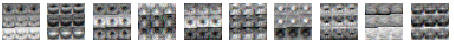
\includegraphics[width=15cm]{img/weights3.png}
\\
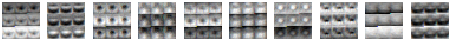
\includegraphics[width=15cm]{img/weights4.png}
\caption{The learned weights for each of the parameter sets in Table \ref{results}. Each row corresponds to a row in this figure.}
\label{weights}
\end{figure}

	
\end{document}